\documentclass{article}
\usepackage[polish]{babel}
\usepackage[OT4]{fontenc}
\usepackage[utf8]{inputenc}
\usepackage{hyperref}
\usepackage{graphicx}
\usepackage{float}
\usepackage{amsmath}
\usepackage{indentfirst}
\usepackage{pythonhighlight}
\title{\textbf{Praca projektowa z przedmiotu Sztuczna Inteligencja}}
\author{Bartłomiej Czajka 169522 2 EF-DI P1}
\date{Rzeszów, 2023}
\linespread{1.5}
\begin{document}
\maketitle
\pagebreak


\tableofcontents{}
\newpage
\section{Opis projektu}
\subsection{Założenia projektowe}
Celem projektu jest realizacja sieci neuronowej uczonej za pomocą sieci głębokiej, klasyfikującej chorobę Parkinsona oraz zbadanie wpływu parametrów sieci na proces uczenia.
Projekt został zrealizowany w języku Python z wykorzystaniem biblioteki PyTorch.
\subsection{Zestaw danych}
Zestaw danych uczących został pobrany ze strony \href{http://archive.ics.uci.edu/ml/datasets/Parkinsons}{http://archive.ics.uci.edu/ml/datasets/Parkinsons}.
Zawiera on 197 instancji, 23 cechy oraz 2 klasy. Dane są nieuporządkowane, nie ma danych nieokreślonych.
Dokładniejszy opis cech zestawu:
\begin{itemize}
    \item name - Nazwa badanego pacjenta w ASCII i numer nagrania.
    \item MDVP:Fo(Hz) - Średnia częstotliwość podstawowa głosu.
    \item MDVP:Fhi(Hz) - Maksymalna częstotliwość podstawowa głosu.
    \item MDVP:Flo(Hz) - Minimalna częstotliwość podstawowa głosu.
    \item MDVP:Jitter(\%), MDVP:Jitter(Abs), MDVP:RAP, MDVP:PPQ, Jitter:DDP - Kilka miar zmienności częstotliwości podstawowej.
    \item MDVP:Shimmer, MDVP:Shimmer(dB), Shimmer:APQ3, Shimmer:APQ5, MDVP:APQ, Shimmer:DDA - Kilka miar zmienności amplitudy.
    \item NHR, HNR - Dwie miary stosunku szumu do składowych tonalnych w głosie.
    \item status - Stan zdrowia badanego (jeden) - chory na Parkinsona, (zero) - zdrowy.
    \item RPDE, D2 - Dwie miary złożoności dynamicznej nieliniowej.
    \item DFA - Wykładnik skalowania fraktalnego sygnału.
    \item spread1, spread2, PPE - Trzy nieliniowe miary zmienności częstotliwości podstawowej.
\end{itemize}
\subsection{Przygotowanie danych}
Sieć ma za zadanie sklasyfikować czy pacjent cierpi na chorobę Parkinsona. Wartość '1' oznacza osobę cierpiącą na chorobę Parkinsona, natomiast '0' oznacza osobę zdrową.
Dane zostały uporządkowane i znormalizowane.
Normalizacja została wykonana dla każdej obserwacji przy użyciu wzoru:
\[
    x_{\text{norm}} = \frac{{x_{\text{norm\_max}} - x_{\text{norm\_min}}}}{{x_{\text{max}} - x_{\text{min}}}} \cdot (x - x_{\text{min}}) + x_{\text{norm\_min}}
\]

gdzie:
\begin{itemize}
    \item $x_{min}$ - to wektor zawierający minimalne wartości dla każdej obserwacji.
    \item $x_{max}$ - to wektor zawierający maksymalne wartości dla każdej obserwacji.
    \item $x_{norm\_min}$ - to wartość minimalna po normalizacji (-1).
    \item $x_{norm\_max}$ - to wartość maksymalna po normalizacji (1).
    \item $x_{norm}$ - to macierz zawierająca znormalizowane dane.
    \item $x$ - to macierz zawierająca dane wejściowe.
\end{itemize}
\newpage
\section{Zagadnienia teoretyczne}
\subsection{Matematyczny opis sztucznego neuronu}
Podstawowym elementem budującym strukturę sieci neuronowej jest neuron. Jest to element, który przetwarza informacje.
W pewnym, uproszczonym stopniu jest wzorowany na funkcjonowaniu biologicznej komórki nerwowej.
Struktura neuronu zawiera wiele wejść oraz jedno wyjście.
Jednym z najważniejszych składników neuronu są wagi, których wartości decydują o zachowaniu neuronu. Są one zazwyczaj ustalane w trakcie procesu uczenia.

\begin{figure}[H]
    \centering
    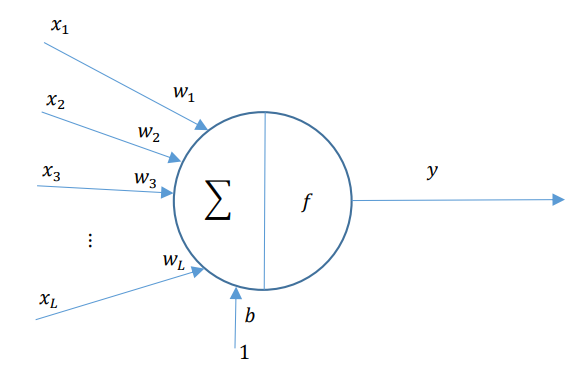
\includegraphics[width=0.8\textwidth, keepaspectratio]{model_neuronu.png}
    \caption{Model neuronu [3]}
    \label{fig:zdjecie}
\end{figure}

Każdy pojedynczy neuron przyjmuje sygnały wejściowe, które są następnie przetwarzane.
Każde wejście ma przypisany współczynnik wagowy, który określa jak bardzo wpływa ono na wynik neuronu.
Ponadto, neuron posiada "bias", czyli dodatkowe wejście, na którym występuje stała wartość.
Wszystkie te informacje są sumowane, aby obliczyć łączne pobudzenie neuronu.
Następnie wartość pobudzenia przechodzi przez funkcję aktywacji, która określa sygnał wyjściowy neuronu.

Wzór na łączne pobudzenie neuronu:
\[
    y = \sum_{j=1}^{L} f(w_{j} x_{j} + b)
\]

gdzie:
\begin{itemize}
    \item $j$ -- indeks, który przyjmuje wartości od 1 do $L$,
    \item $y$ -- wyjście neuronu,
    \item $w_{j}$ -- współczynnik wagowy przypisany do $j$-tego wejścia,
    \item $x_{j}$ -- $j$-ty sygnał wejściowy,
    \item $b$ -- bias [2].
\end{itemize}

\subsection{Funkcja aktywacji}
Sam model matematyczny neuronu nie byłby wystarczający do skomplikowanych obliczeń w m.in. sieciach głębokich.
Należy wprowadzić funkcje aktywacji, które nadają sieciom neuronowym zdolność modelowania nieliniowych relacji między danymi wejściowymi, a wyjściowymi.
Dzięki tej nieliniowej transformacji na wyjściu sztucznego neuronu, możliwe jest wprowadzenie nieliniowości i bardziej skomplikowanych obliczeń.

Istnieje wiele funkcji aktywacji.
Szczególnie przydatną w modelach głębokich ze względu na swoją prostotę i skuteczność jest funkcja ReLU, która została przeze mnie wykorzystana jako funkcja aktywacji dla warstw ukrytych.
Działa na zasadzie przekazywania wartości dodatnich bez ich zmiany, natomiast dla wartości ujemnych przypisuje zerową wartość.
Matematycznie można zdefiniować ją następującym wzorem:
\[
    f(x) = \max(0, x)
\]
Innymi słowy, funkcja ReLU jest zdefiniowana na przedziale:
\[
    f(x) = \begin{cases}
        0, & \text{gdy } x \leq 0, \\
        x, & \text{gdy } x > 0.
    \end{cases}
\]
gdzie:
\begin{itemize}
    \item $x$ -- wartość wejściowa, na której zostanie zastosowana funkcja aktywacji.
\end{itemize}

Istnieje również funkcja aktywacji softmax, która dla danego wektora wyników \( \mathbf{z} = (z_1, z_2, \ldots, z_n) \), gdzie \( n \) oznacza liczbę klas, przekształca każdy element \( z_i \) na wartość prawdopodobieństwa \( p_i \).

Funkcję softmax można zdefiniować w następujący sposób:
\[
    f(z)_i = \frac{e^{z_i}}{\sum_{j=1}^{n} e^{z_j}}
\]
gdzie:
\begin{itemize}
    \item \(f(z)_i\) -- \(i\)-ty element wyniku funkcji softmax dla wektora wyników \(\mathbf{z}\),
    \item \(e^{z_i}\) -- funkcja wykładniczą podniesiona do potęgi \(z_i\),
    \item \(z_i\) -- \(i\)-ty element wektora wyników,
    \item \(\sum_{j=1}^{n} e^{z_j}\) -- suma funkcji wykładniczych dla wszystkich elementów wektora wyników,
    \item \(n\) -- liczba klas.
\end{itemize}

Kolejną funkcją aktywacji jest funkcja sigmoidalna.
Funkcja sigmoidalna przekształca wartość wejściową na wartość z zakresu (0; 1), co czyni ją przydatną w problemach klasyfikacji binarnej.

Matematycznie funkcję sigmoidalną można zdefiniować jako:
\[
    f(x) = \frac{1}{1 + e^{-x}}
\]
gdzie:
\begin{itemize}
    \item \(x\) -- wartość wejściowa do funkcji sigmoidalnej,
    \item \(e\) --  podstawa logarytmu naturalnego, przybliżone do wartości 2.71828,
    \item \(f(x)\) -- wartość wyjściowa funkcji sigmoidalnej, przekształcająca \(x\) na wartość z przedziału (0; 1).
\end{itemize}

Ostatnią funkcją aktywacji, którą wykorzystałem jest tangens hiperboliczny.
Funkcja ta może zostać użyta zarówno do warstw ukrytych jak i warstwy ostatniej.
Oto jej definicja:
\[\text{tanh}(x) = \frac{{\exp(x) - \exp(-x)}}{{\exp(x) + \exp(-x)}}\]
Wartości tej funkcji mieszczą się w zakresie (-1; 1).
Funkcja kształtem przypomina funkcję sigmoidalną.
Warto wspomnieć o tym, że tangens hiperboliczny jest bardziej wrażliwy na duże wartości wejściowe niż funkcja sigmoidalna, co może prowadzić do problemów z gradientem w czasie uczenia sieci.

\newpage
\subsection{Sieć głęboka}
Sieci głębokie to rodzaj modeli uczenia maszynowego, które składają się z wielu warstw neuronów, zwanych warstwami głębokimi.
Uczenie sieci głębokich opiera się na zasadzie propagacji wstecznej, która jest jednym z kluczowych algorytmów używanych do dostosowania wag sieci neuronowej w procesie uczenia.
Propagacja wsteczna umożliwia obliczenie gradientów wag sieci na podstawie funkcji kosztu i propaguje te gradienty wstecz przez sieć, aby zaktualizować wagi w celu minimalizacji błędu.

\begin{figure}[H]
    \centering
    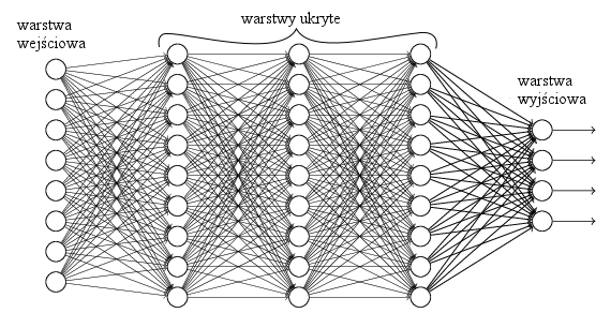
\includegraphics[width=1\textwidth, keepaspectratio]{siec_gleboka.png}
    \caption{Sieć głęboka [5]}
    \label{fig:siec}
\end{figure}

Proces uczenia sieci głębokich rozpoczyna się od inicjalizacji wag, które mogą być inicjalizowane losowo lub przy użyciu innych metod.
Następnie dane wejściowe są przekazywane od warstwy wejściowej do warstwy wyjściowej (ang. forward propagation).
Każda warstwa na podstawie wag i funkcji aktywacji oblicza swoje wyjście.
Na podstawie wyników obliczana jest wartość funkcji kosztu, która mierzy błąd przewidywań sieci.
Kolejnym krokiem jest wykorzystanie algorytmu propagacji wstecznej, który oblicza gradienty wag sieci neuronowej.
Gradienty oblicza się iteracyjnie, zaczynając od warstwy wyjściowej przechodząc wstecz przez kolejne warstwy sieci.
W dalszej kolejności, biorąc pod uwagę obliczone gradienty wag, wagi sieci są aktualizowane w celu zminimalizowania funkcji kosztu mierzącej błąd predykcji sieci.
Dokonuje się tego za pomocą optymalizatora (np. ADAM).
Wyżej wymienione kroki powtarza się aż do osiągnięcia zdefiniowanej liczby epok lub innych kryteriów zatrzymania.
\subsection{Funkcja kosztu}
Wykorzystaną funkcją kosztu w programie jest entropia krzyżowa.
Funkcja ta mierzy stopień niezgodności między rzeczywistymi etykietami, a przewidywanymi prawdopodobieństwami dla każdej klasy.
Im większa niezgodność, tym większa wartość funkcji kosztu.
Dąży się do minimalizacji tej funkcji, poprzez zmianę wag sieci.

Entropię krzyżową, w szczególności dla klasyfikacji binarnej, można zdefiniować następującym wzorem:
\begin{align*}
    H(y, p) & = -\sum_{i=1}^{C} y_i \log(p_i) =    \\
            & = -\sum_{i=1}^{2} y_i \log(p_i) =    \\
            & = -[y_1 \log(p_1) + y_2 \log(p_2)] = \\
            & = - [y \log(p) + (1-y) \log(1-p)]
\end{align*}

gdzie:
\begin{itemize}
    \item  \(H(y, p)\) -- wartość entropii krzyżowej,
    \item  \(y_i\) -- \(i\)-ta rzeczywista etykieta (0 lub 1) dla próbki i,
    \item  \(p_i\) -- \(i\)-te przewidziane prawdopodobieństwo dla próbki i,
    \item \(C\) -- liczba klas.
\end{itemize}

\subsection{Algorytm wstecznej propagacji błędu}
Algorytm wstecznej propagacji błędu, nazywany również algorytmem największego spadku gradientu, jest jednym z głównych algorytmów stosowanych w procesie uczenia sieci głębokich.
Umożliwia on aktualizację wag sieci w celu minimalizacji funkcji kosztu poprzez iterację przez kolejne warstwy sieci.
Proces ten można podzielić na dwa kroki: propagację w przód oraz wstecz.

Propagacja w przód polega na przekazywaniu danych wejściowych przez sieć od warstwy wejściowej do warstwy wyjściowej.
W każdej warstwie obliczane są aktywacje neuronów na podstawie obecnych wag i danych wejściowych.
Wyniki z danej warstwy przekazywane są do kolejnej aż do warstwy wyjściowej gdzie generowany jest wynik predykcji.

W propagacji wstecznej natomiast porównuje się wynik sieci z oczekiwanym wynikiem, obliczając przy tym błąd.
Błąd ten jest następnie propagowany wstecz od zaczynając od warstwy wyjściowej.
Obliczany jest gradient funkcji kosztu względem wag sieci, który informuje o kierunku dostosowania wag w celu minimalizacji błędu.
Na podstawie gradientu aktualizowane są wagi sieci przy użyciu odpowiedniej metody optymalizacji, takiej jak metoda spadku gradientu czy też jej wariant, np. ADAM.

\subsection{Metoda optymalizacji ADAM}
Metoda ADAM jest popularna w optymalizacji sieci głębokich, ponieważ łączy zalety adaptacyjnego skalowania kroku uczenia (RMSProp) i momentu, co prowadzi do efektywniejszej optymalizacji i szybszego zbiegania do optymalnych wag sieci.

Aby obliczyć gradient funkcji kosztu, należy obliczyć pochodne cząstkowe dla każdej warstwy, od ostatniej do pierwszej.
W każdej warstwie oblicza się lokalny gradient na podstawie pochodnej funkcji kosztu oraz gradientu z poprzedniej warstwy.

Wzór na gradient funkcji kosztu H, w kroku t:
\[ g_t = \frac{\partial H}{\partial W} \]
gdzie:
\begin{itemize}
    \item \( H\) -- funkcja kosztu,
    \item \(W\) -- macierz wag sieci neuronowej.
\end{itemize}

Algorytm ADAM składa się z następujących kroków:
\begin{enumerate}
    \item Obliczenie gradientów funkcji kosztu względem wag sieci za pomocą propagacji wstecznej błędu.
    \item Aktualizacja momentu gradientu \(m_t\) i drugiego momentu gradientu \(v_t\) na podstawie obliczonych gradientów.
    \item Obliczenie wygładzonych estymacji momentu i drugiego momentu: \(\hat{m}_t\) i \(\hat{v}_t\).
    \item Aktualizacja wag sieci z wykorzystaniem estymacji momentu i drugiego momentu, współczynnika uczenia \(\alpha\) oraz małej wartości epsilon \(\epsilon\).
\end{enumerate}

Gradient jest używany do aktualizacji wag zgodnie z następującymi wzorami:
\[m_t = \beta_1 \cdot m_{t-1} + (1 - \beta_1) \cdot g_t\]
\[v_t = \beta_2 \cdot v_{t-1} + (1 - \beta_2) \cdot g_t^2\]
\[\hat{m}_t = \frac{m_t}{1 - \beta_1^t}\]
\[\hat{v}_t = \frac{v_t}{1 - \beta_2^t}\]
\[ W_{t+1} = W_t - \frac{\eta}{\sqrt{\hat{v}_t} + \epsilon} \cdot \hat{m}_t \]
gdzie:
\begin{itemize}
    \item \(m_t\) to estymacja momentu gradientu w kroku czasowym \(t\),
    \item \(v_t\) to estymacja drugiego momentu gradientu w kroku czasowym \(t\),
    \item \(\beta_1\) i \(\beta_2\) to współczynniki z zakresu \([0; 1)\) kontrolujące eksponencjalne wygładzanie momentu i drugiego momentu,
    \item \(\alpha\) to współczynnik uczenia,
    \item \(\epsilon\) to mała wartość (np. \(10^{-10}\)) używana w celu uniknięcia dzielenia przez zero,
    \item \(\hat{m}_t\) i \(\hat{v}_t\) to wygładzone estymacje momentu i drugiego momentu,
    \item \(W_{t}\) i \(W_{t+1}\) to wagi w krokach czasowych \(t\) i \(t+1\).
\end{itemize}

Przy użyciu tych wzorów, w metodzie optymalizacji ADAM aktualizuje się wagi sieci neuronowej, wykorzystując estymację momentu i drugiego momentu gradientu.
To pozwala na efektywną optymalizację sieci głębokiej, dostosowując krok uczenia dla każdej wagi indywidualnie.

\newpage
\section{Realizacja sieci neuronowej}
\subsection{Opis skryptu}

Główny skrypt został podzielony na kilka innych w zależności od zastosowania.
Każdy z nich dotyczy tego jak zmienia się poprawność klasyfikacji w zależności od różnych parametrów.
Wszystkie skrypty mają taką samą wspólną, początkową część, która zawiera przetwarzanie danych zawartych w pliku `parkinsons.txt'.
Dane podlegają normalizacji, sortowaniu i zapisaniu do pliku `parkinsons.hkl'.
Następnie dane wejściowe są skalowane i dzielone na zbiór treningowy oraz testowy.
Wektory `y' są przekształcane tak, aby indeks pierwszej klasy wynosił 0.
Dalsza część kodu jest inna dla każdego ze skryptów.

\subsection{Początek każdego ze skryptów [5]}
\begin{verbatim}
    from torch.autograd import Variable
    import torch.nn as nn
    import torch.nn.functional as F
    import torch
    import numpy as np
    import matplotlib.pyplot as plt
    import hickle as hkl
    from sklearn.model_selection import train_test_split
    from sklearn.preprocessing import StandardScaler
    
    """Data preparation with manual deletion of the first line (feature names)"""
    filename = "parkinsons.txt"
    data = np.loadtxt(filename, delimiter=",", dtype=str)
    x = np.concatenate((data[:, 1:17], data[:, 18:]), axis=1).astype(float).T
    y_t = data[:, 17].astype(float)
    y_t = y_t.reshape(1, y_t.shape[0])
    np.transpose([np.array(range(x.shape[0])), x.min(axis=1), x.max(axis=1)])
    
    # Normalization
    x_min = x.min(axis=1)
    x_max = x.max(axis=1)
    x_norm_max = 1
    x_norm_min = -1
    x_norm = np.zeros(x.shape)
    for i in range(x.shape[0]):
        x_norm[i, :] = (x_norm_max - x_norm_min) / (x_max[i] - x_min[i]) * (
            x[i, :] - x_min[i]
        ) + x_norm_min
    np.transpose([np.array(range(x.shape[0])),
                 x_norm.min(axis=1), x_norm.max(axis=1)])
    
    # Before sorting
    plt.plot(y_t[0])
    # plt.show()
    
    y_t_s_ind = np.argsort(y_t)
    x_n_s = np.zeros(x.shape)
    y_t_s = np.zeros(y_t.shape)
    for i in range(x.shape[1]):
        y_t_s[0, i] = y_t[0, y_t_s_ind[0, i]]
        x_n_s[:, i] = x_norm[:, y_t_s_ind[0, i]]
    
    # After sorting
    plt.plot(y_t_s[0])
    # plt.show()
    
    hkl.dump([x, y_t, x_norm, x_n_s, y_t_s], "parkinsons.hkl")
    x, y_t, x_norm, x_n_s, y_t_s = hkl.load("parkinsons.hkl")
    if min(y_t.T)[0] > 0:
        y = y_t.squeeze() - 1  # index of first class should equal to 0
    else:
        y = y_t.squeeze()
    X = x.T
    
    # Scale data to have mean 0 and variance 1
    # which is importance for convergence of the neural network
    scaler = StandardScaler()
    X_scaled = scaler.fit_transform(X)
    
    # Split the data set into training and testing
    X_train, X_test, y_train, y_test = train_test_split(
        X_scaled, y, test_size=0.2, random_state=2
    )
\end{verbatim}

Na początku, przy użyciu funkcji `np.loadtxt()' wczytywane są dane z pliku `parkinsons.txt'.
Tworzona jest macierz `x' poprzez konkatenację dwóch części z `data', aby pozbyć się niepotrzebnej kolumny.
Później macierz `x' jest transponowana i konwertowana do typu `float'.
Następnie tworzony jest wektor `y\_t' i zmieniany jest jego kształt na (1, liczba przykładów).
Kolejno tworzona jest macierz, w której każdy wiersz zawiera indeks, minimalną wartość i maksymalną wartość dla odpowiadającego wiersza macierzy `x'.
Kolejnym etapem jest normalizacja danych.
Obliczane są minimalne oraz maksymalne wartości dla każego wiersza macierzy `x' za pomocą `x\_min = x.min(axis=1)' oraz `x\_max = x.max(axis=1)'.
Później ustalane są minimalne i maksymalne wartości dla normalizacji (-1 oraz 0).
Przeprowadzana jest następnie normalizacja dla każdego wiersza `x[i, :]', a wynik jest zapisywany do macierzy `x\_norm'.
Wykonana zostaje również transpozycja macierzy, która tworzy macierz wynikową, gdzie każdy wiersz zawiera indeks, minimalną wartość i maksymalną wartość dla odpowiadającego wiersza macierzy `x\_norm'.

Dalszym etapem jest stworzenie indeksów, które posortują wartości wektora `y\_t' w kolejności rosnącej.
Utworzona zostaje macierz `x\_n\_s', o takim samym kształcie jak `x'. Zostanie użyta do przechowywania znormalizowanych danych po sortowaniu.
Analogicznie zostaje utworzona macierz `y\_t\_s'
\subsection{Główna część skryptu dla zależności poprawności klasyfikacji od liczby neuronów w warstwach [6]}
\begin{verbatim}
class Model(nn.Module):
    def __init__(self, input_dim, output_dim, K1, K2):
        super(Model, self).__init__()
        self.layer1 = nn.Linear(input_dim, K1)
        self.layer2 = nn.Linear(K1, K2)
        self.layer3 = nn.Linear(K2, output_dim)

    def forward(self, x):
        x = F.relu(self.layer1(x))
        x = F.relu(self.layer2(x))
        x = F.sigmoid(self.layer3(x))
        return x

lr_vec = np.array([1e-1, 1e-2, 1e-3, 1e-4, 1e-5, 1e-6, 1e-7])
K1_vec = np.arange(2, 30, 2)
K2_vec = K1_vec
PK_2D_K1K2 = np.zeros([len(K1_vec), len(K2_vec)])
max_epoch = 100
PK_2D_K1K2_max = 0
k1_ind_max = 0
k2_ind_max = 0
X_train = Variable(torch.from_numpy(X_train)).float()
y_train = Variable(torch.from_numpy(y_train)).long()
X_test = Variable(torch.from_numpy(X_test)).float()
y_test = Variable(torch.from_numpy(y_test)).long()
for k1_ind in range(len(K1_vec)):
    for k2_ind in range(len(K2_vec)):
        model = Model(X_train.shape[1], int(
            max(y) + 1), K1_vec[k1_ind], K2_vec[k2_ind])
        optimizer = torch.optim.Adam(model.parameters(), lr=lr_vec[0])
        loss_fn = nn.CrossEntropyLoss()

        for epoch in range(max_epoch):
            y_pred = model(X_train)
            loss = loss_fn(y_pred, y_train)

            optimizer.zero_grad()
            loss.backward()
            optimizer.step()

        with torch.no_grad():
            y_pred = model(X_test)
            correct = (torch.argmax(y_pred, dim=1) ==
                       y_test).type(torch.FloatTensor)
            PK = correct.mean().item() * 100
            print("K1 {} | K2 {} | PK {} ".format(
                K1_vec[k1_ind], K2_vec[k2_ind], PK))
            PK_2D_K1K2[k1_ind, k2_ind] = PK

        if PK > PK_2D_K1K2_max:
            PK_2D_K1K2_max = PK
            k1_ind_max = k1_ind
            k2_ind_max = k2_ind
\end{verbatim}

Na początku skryptu zostaje zdefiniowana klasa `Model', która dziedziczy po module `nn.Module'.
Jest to model sieci neuronowej.
Jej konstruktor przyjmuje $4$ argumenty (rozmiar wejścia, rozmiar wyjścia, rozmiar warstwy pierwszej, rozmiar warstwy drugiej).
W konstruktorze klasy zostaje zdefiniowana struktura modelu, tzn. warstwy liniowe `nn.Linear' i ich rozmiary.
Pierwsza warstwa ma rozmiar `input\_dim' na `K1', druga warstwa `K1' na `K2', a trzecia `K2' na `output\_dim'.

W klasie zostaje również zdefiniowana metoda `forward', która definiuje przepływ danych przez model.
Przyjmuje jeden argument `x', który jest wejściem do modelu.
Działanie tej metody polega na przekazywaniu wejścia `x' przez warstwę pierwszą, stosując następnie funkcję aktywacji ReLU.
Wynik przekazywany jest do kolejnej warstwy i ponownie stosuje się tą samą funkcję aktywacji.
Na końcu wynik jest przekazywany przez ostatnią warstwę i poddawany funkcji sigmoidalnej.
Ostatecznie wynik jest zwracany jako wyjście modelu.

Metoda wykorzystuje funkcje aktywacji ReLU oraz funkcję softmax na ostatniej warstwie.
Później następuje definicja parametrów uczenia, których opis znajduje się poniżej:
\begin{itemize}
    \item \texttt{lr\_vec} -- wektor współczynników uczenia,
    \item \texttt{K1\_vec} oraz \texttt{K2\_vec} -- wektory, które odpowiadają rozmiarom warstw w modelu. Generowane są przy wykorzystaniu \texttt{np.arange},
    \item \texttt{PK\_2D\_K1K2} -- macierz, która będzie przechowywać wyniki ocenu modelu dla różnych kombinacji,
    \item \texttt{max\_epoch} -- oznacza maksymalną liczbę epok,
    \item \texttt{PK\_2D\_K1K2\_max} -- dotychczasowa maksymalna poprawność klasyfikacji,
    \item \texttt{k1\_ind\_max}, \texttt{k2\_ind\_max} -- indeksy kombinacji rozmiarów warstw odpowiednio \texttt{K1} oraz \texttt{K2}, dla których uzyskano najwyższą ocenę \texttt{PK\_2D\_K1K2\_max},
    \item \texttt{X\_train}, \texttt{y\_train} -- dane treningowe, przekształcone do zmiennych tensorowych,
    \item \texttt{X\_test}, \texttt{y\_test} -- dane testowe, przekształcone do zmiennych tensorowych.
\end{itemize}

Zagnieżdżone pętle `for' iterują po rozmiarach `K1' oraz `K2'.
Tworzony jest model z odpowiednimi rozmiarami warstw.
Dwa pierwsze parametry przekazane do modelu to:
\begin{itemize}
    \item X\_train.shape[1] -- rozmiar wejścia (ilość cech) dla danych treningowych zwrócone jako krotka,
    \item int(max(y) + 1) -- rozmiar wyjścia modelu, gdzie max(y) zwraca maksymalną wartość w wektorze etykiet `y'. Dodanie jedynki jest istotne, gdyż numery klas są indeksowane od zera. Po dodaniu jedynki liczba klas jest odzwierciedlona poprawnie.
\end{itemize}


Następnie definiowany jest optymalizator `ADAM' oraz funkcja kosztu.
W pętli treningowej obliczane są predykcje modelu (`y\_pred') dla danych treningowych, wartość funkcji kosztu na podstawie przewidywań `y\_pred' i etykiet `y\_train'.
Kolejnym krokiem jest zresetowanie gradientów optymalizatora (`optimizer\_zero\_grad()'), obliczenie gradientów funkcji straty (`loss.backward()') oraz zaktualizowanie wag modelu (`optimizer\_step()').

Po zakończeniu treningu następuje część kodu, która wyłącza obliczanie gradientów dla testowania modelu (`with torch.no\_grad()').
W tej części obliczane są przewidywane wartości `y\_pred' dla danych testowych.
Następnie obliczana jest dokładność modelu na podstawie porównania przewidywanych etykiet z rzeczywistymi etykietami.
Wywołanie funkcji `torch.argmax(y\_pred, dim=1)' oblicza indeksy klas o najwyższych wartościach dla każdego przykładu w `y\_pred' wzdłuż określonego wymiaru (1), co oznacza drugi wymiar, czyli klasę.
Indeksy porównywane są z rzeczywistymi etykietami `y\_test'.
Na końcu obliczana jest ocena `PK' dla danych testowych, na podstawie obliczonej dokładności.
Jeżeli aktualna poprawność klasyfikacji jest większa od dotychczasowej, maksymalnej, aktualizowane są odpowiednie zmienne.

\subsection{Główna część skryptu dla zależności poprawności klasyfikacji od liczby warstw oraz współczynnika uczenia [6]}
\begin{verbatim}
class Model(nn.Module):
    def __init__(self, input_dim, output_dim, K):
        super(Model, self).__init__()
        layers = [nn.Linear(input_dim, K[0])]
        for i in range(len(K) - 1):
            layers.append(nn.Linear(K[i], K[i + 1]))
        layers.append(nn.Linear(K[-1], output_dim))
        self.layers = nn.ModuleList(layers)

    def forward(self, x):
        for layer in self.layers[:-1]:
            x = F.relu(layer(x))
        x = F.sigmoid(self.layers[-1](x))
        return x

lr_vec = np.array([1e-1, 1e-2, 1e-3, 1e-4, 1e-5, 1e-6, 1e-7])
K1 = 6
K2 = 4
max_layers = 10
PK_3D_K = np.zeros((len(lr_vec), max_layers))
max_epoch = 100
PK_max = 0
lr_max_ind = 0
layers_for_max_PK = 0

X_train = Variable(torch.from_numpy(X_train)).float()
y_train = Variable(torch.from_numpy(y_train)).long()
X_test = Variable(torch.from_numpy(X_test)).float()
y_test = Variable(torch.from_numpy(y_test)).long()

for lr_ind in range(len(lr_vec)):
    for i in range(3, max_layers + 1):
        layers = []
        for j in range(i):
            if j % 2 == 0:
                layers.append(K1)
            else:
                layers.append(K2)
        model = Model(X_train.shape[1], int(max(y) + 1), layers)
        optimizer = torch.optim.Adam(model.parameters(), lr=lr_vec[lr_ind])
        loss_fn = nn.CrossEntropyLoss()

        for epoch in range(max_epoch):
            y_pred = model(X_train)
            loss = loss_fn(y_pred, y_train)

            optimizer.zero_grad()
            loss.backward()
            optimizer.step()

        with torch.no_grad():
            y_pred = model(X_test)
            correct = (torch.argmax(y_pred, dim=1) == y_test).type(torch.FloatTensor)
            PK = correct.mean().item() * 100
            print(
                "LR {} | K1 {} | K2 {} | PK {} | layers {} | layers_count {} ".format(
                    lr_vec[lr_ind], K1, K2, PK, layers, len(layers)
                )
            )
            PK_3D_K[lr_ind, i - 3] = PK

        if PK > PK_max:
            PK_max = PK
            lr_max_ind = lr_ind
            layers_for_max_PK = len(layers)

print(
    "Max PK: {} for LR: {} | K1: {} | K2: {} | layers_count {} ".format(
        PK_max, lr_vec[lr_max_ind], K1, K2, layers_for_max_PK
    )
)

\end{verbatim}
\newpage
Względem poprzedniego skryptu, klasa `Model' uległa zmianie.
Konstruktor tej klasy inicjalizuje kolejne warstwy sieci, na podstawie przekazanej listy `K'.
Lista `K' zawiera liczbę neuronów dla poszczególnych warstw.
Występują również dwie zagnieżdżone pętle, które iterują po liczbie warstw z zakresu 3 - 10 oraz po współczynniku uczenia z zakresu $10^{-1}$ - $10^{-7}$.
Założono, że liczba neuronów w danej warstwie będzie wynosić `K1', jeżeli numer warstwy jest parzysty oraz `K2' w przeciwnym wypadku.

\subsection{Główna część skryptu dla zależności poprawności klasyfikacji od użytej funkcji aktywacji [6]}
\begin{verbatim}
class Model(nn.Module):
    def __init__(self, input_dim, output_dim, K, activation):
        super(Model, self).__init__()
        layers = [nn.Linear(input_dim, K[0])]
        for i in range(len(K) - 1):
            layers.append(nn.Linear(K[i], K[i+1]))
        layers.append(nn.Linear(K[-1], output_dim))
        self.layers = nn.ModuleList(layers)
        self.activation = activation

    def forward(self, x):
        for layer in self.layers[:-1]:
            x = self.activation(layer(x))
        x = F.softmax(self.layers[-1](x), dim=1)
        return x

activations = [F.relu, F.tanh, F.sigmoid]
PK_activations = []
X_train = Variable(torch.from_numpy(X_train)).float()
y_train = Variable(torch.from_numpy(y_train)).long()
X_test = Variable(torch.from_numpy(X_test)).float()
y_test = Variable(torch.from_numpy(y_test)).long()

layers = 2
K = [6, 4]
max_epoch = 100
lr_vec = np.array([1e-1, 1e-2, 1e-3, 1e-4, 1e-5, 1e-6, 1e-7])
for activation in activations:
    model = Model(X_train.shape[1], int(max(y) + 1), K, activation)
    optimizer = torch.optim.Adam(model.parameters(), lr=lr_vec[0])
    loss_fn = nn.CrossEntropyLoss()

    for epoch in range(max_epoch):
        y_pred = model(X_train)
        loss = loss_fn(y_pred, y_train)

        optimizer.zero_grad()
        loss.backward()
        optimizer.step()

    with torch.no_grad():
        y_pred = model(X_test)
        correct = (torch.argmax(y_pred, dim=1) == y_test).type(torch.FloatTensor)
        PK = correct.mean().item() * 100
        PK_activations.append(PK)
        print("PK {} FUNCTION {}".format(PK, activation))

\end{verbatim}

Konstruktor klasy `Model' został uzupełniony o przekazywaną funkcję aktywacji.
W kodzie pojawiła się również lista `activations', która zawiera funkcje aktywacji takie jak ReLU, tangens hiperboliczny oraz funkcję sigmoidalną.
Dalsza część skryptu polega na iteracji po tej liście.
Obliczana jest maksymalna poprawność klasyfikacji w zależności od użytej funkcji aktywacji.

\newpage
\section{Eksperymenty}
Dla każdego eksperymentu został użyty nieco inny skrypt.
Pierwsze eksperymenty dotyczą rozmiaru warstw dla sieci trójwarstwowej, natomiast kolejne dotyczą zmian współczynniku uczenia, liczby warstw oraz funkcji przejścia.

\newpage
\subsection{Eksperyment 1}

Eksperyment pierwszy został przeprowadzony dla przykładowych liczb neuronów będących wielokrotnościami liczby 2.
Warstwy pierwsza i druga zawierają liczbę neuronów z zakresu 2 - 28.
Współczynnik uczenia wynosi $0.1$, natomiast liczba epok to $1000$.

\begin{figure}[H]
    \centering
    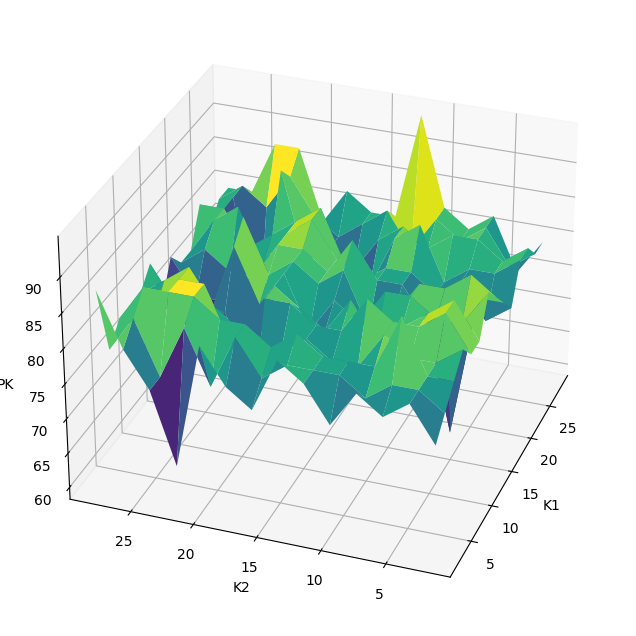
\includegraphics[width=0.8\textwidth, keepaspectratio]{k1_k2_dobre_1_1000echo.png}
    \caption{Zależność poprawności klasyfikacji od liczby neuronów z zakresu 2-28 z krokiem 2}
    \label{fig:k1k2_1}
\end{figure}

Dla danych metaparametrów wykres jest dosyć chaotyczny.
Dominującą wartością poprawności klasyfikacji jest $79.48\%$, natomiast najlepszą wartość ($94.87\%$) uzyskano dla `K1' = 28, `K2' = 12.

\newpage
\subsection{Eksperyment 2}
Tym razem warstwa pierwsza i druga zawierają liczbę neuronów z zakresu 100 - 900, które są wielokrotnościami liczby 100.
Liczba epok wynosi 100, natomiast współczynnik uczenia pozostał niezmieniony i wynosi $0.1$.
\begin{figure}[H]
    \centering
    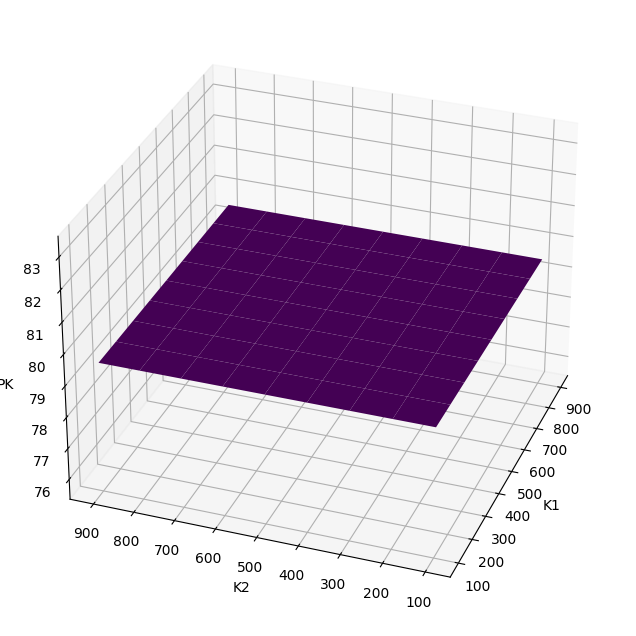
\includegraphics[width=0.8\textwidth, keepaspectratio]{k1_k2_dobre_900k1k2_echo100.png}
    \caption{Zależność poprawności klasyfikacji od liczby neuronów z zakresu 100-900 z krokiem 100}
    \label{fig:k1k2_2}
\end{figure}

Sieć uczyła się zdecydowanie dłużej.
Okazało się, że wykres jest płaski dla większej liczby neuronów.
Skrypt został uruchomiony ponownie kilkukrotnie, wynik był jednak identyczny.
Oznacza to, że zwiększanie liczby neuronów w tym przypadku nie ma żadnego wpływu na poprawność klasyfikacji, która wynosi $79.48\%$.

\newpage
\subsection{Eksperyment 3}
Plan trzeciego eksperymentu zakłada zweryfikowanie, czy dla liczby neuronów z zakresu 100 - 900, które tym razem są wielokrotnościami liczby 50 wykres będzie podobny.
Zmieniona zostanie liczba epok (1000), a współczynnik uczenia będzie dalej wynosić $0.1$.

\begin{figure}[H]
    \centering
    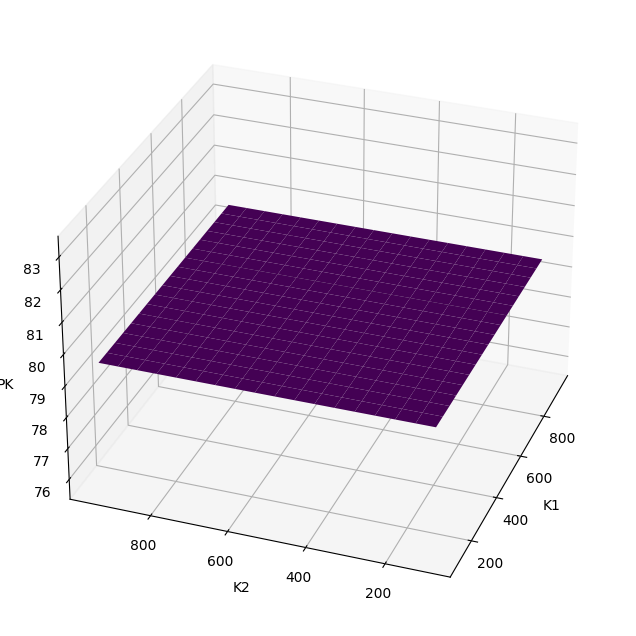
\includegraphics[width=0.8\textwidth, keepaspectratio]{k1_k2_dobre_3_950_50.png}
    \caption{Zależność poprawności klasyfikacji od liczby neuronów z zakresu 100-900 z krokiem 50}
    \label{fig:k1k2_3}
\end{figure}

Sieć uczyła się jeszcze dłużej względem eksperymentu drugiego.
Jak widać na powyższym rysunku, wykres wygląda identycznie nawet jeżeli zostanie zwiększona liczba epok oraz krok zmiany liczby neuronów.
Dominuje poprawność klasyfikacji na poziomie $79.48\%$, tak jak w poprzednim eksperymencie.

\newpage
\subsection{Eksperyment 4}
Eksperyment czwarty będzie polegał na zmianie liczby warstw oraz współczynniku uczenia sieci.
W tym celu użyto innego skryptu niż ten wykorzystany w poprzednich eksperymentach.
Liczba neuronów wynosi 6, jeżeli indeks warstwy jest parzysty oraz 4 w przeciwnym wypadku.
Liczba epok została ustawiona na 100, a maksymalna liczba warstw, na których będą przeprowadzane testy, wynosi 10.

\begin{figure}[H]
    \centering
    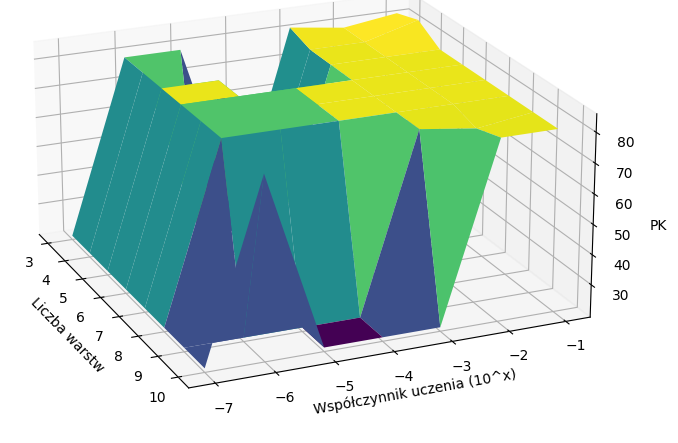
\includegraphics[width=0.8\textwidth, keepaspectratio]{LR_LAYERS_100ECHO.PNG}
    \caption{Zależność poprawności klasyfikacji od liczby warstw i współczynniku uczenia}
    \label{fig:lr_layers_1}
\end{figure}

Dla zmniejszającego się współczynnika uczenia, sieć zachowuje się bardziej nieprzewidywalnie.
Z wykresu wynika, że liczba warstw nie ma tak dużego wpływu na uczenie się sieci.
Znowu dominuje poprawność klasyfikacji na poziomie około $79\%$.
Możliwe, że liczba 100 epok jest niewystarczająca.
Kolejny eksperyment to zweryfikuje.

\newpage
\subsection{Eksperyment 5}
Eksperyment będzie przeprowadzony w sposób analogiczny do poprzedniego, ale liczba epok zostanie zwiększona do 3000.
\begin{figure}[H]
    \centering
    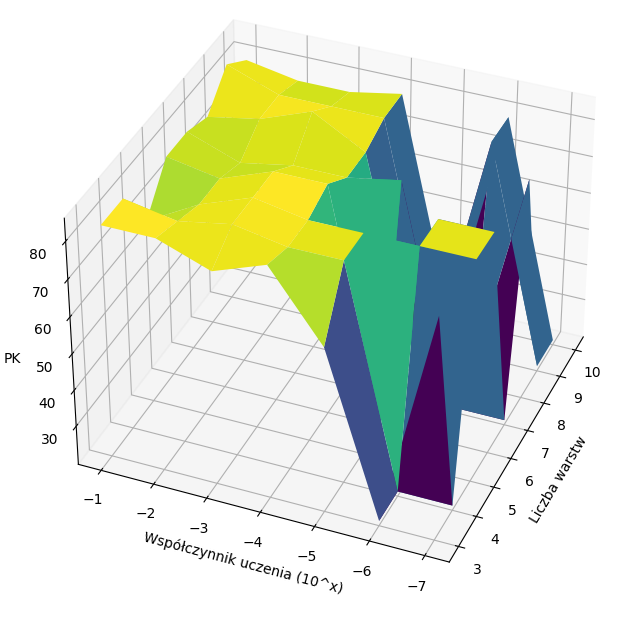
\includegraphics[width=0.8\textwidth, keepaspectratio]{LR_LAYERS_3000ECHO.PNG}
    \caption{Zależność poprawności klasyfikacji od liczby warstw i współczynniku uczenia}
    \label{fig:lr_layers_2}
\end{figure}

Przy liczbie warstw większej od 5 oraz współczynniku uczenia mniejszym od $10^{-6}$ sieć wykazuje niestabilne zachowanie.
To zjawisko jest podobne do obserwowanego w poprzednim eksperymencie.
Liczba epok nie ma tu zbyt wielkiego znaczenia.
Najlepszy wynik poprawności klasyfikacji uzyskano przy użyciu 9 warstw i współczynnika uczenia wynoszącego $0.1$, co dało wynik na poziomie $84$\%.

\newpage
\subsection{Eksperyment 6}
Eksperyment ten sprawdzi co się stanie, gdy zwiększymy liczbę neuronów dla `K1' do 1500 oraz `K2' do 1000.
Liczba epok zostanie przywrócona do 100.

\begin{figure}[H]
    \centering
    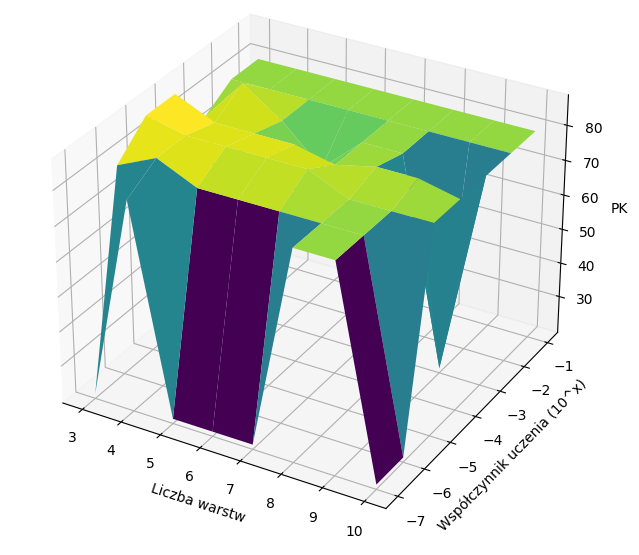
\includegraphics[width=0.8\textwidth, keepaspectratio]{LR_LAYERS_1500_1000K1K2.PNG}
    \caption{Zależność poprawności klasyfikacji od liczby warstw i współczynniku uczenia}
    \label{fig:lr_layers_3}
\end{figure}

Wyniki okazały się być podobne.
W przypadku liczby warstw większej niż 5 oraz współczynnika uczenia mniejszego od $10^{-6}$, sieć nadal wykazuje niestabilne zachowanie.
Dla pozostałych wartości, poprawność klasyfikacji utrzymuje się na identycznym poziomie, wynoszącym około $79\%$.
Najlepszy wynik poprawności klasyfikacji uzyskano przy użyciu 4 warstw i współczynnika uczenia wynoszącego $0.001$, co dało rezultat na poziomie około $87\%$.

\newpage
\subsection{Eksperyment 7}
Tym razem badany będzie wpływ różnych funkcji aktywacji na poprawność klasyfikacji.
Dotychczas w warstwie pierwszej oraz w warstwach ukrytych używana była funkcja ReLU.
W celu porównania, zostaną wykorzystane funkcje aktywacji sigmoidalna oraz tangens hiperboliczny.

Eksperyment zostanie przeprowadzony dla suboptymalnych wartości z pierwszego eksperymentu: `K1' = 6, `K2' = 4, współczynnik uczenia to $0.1$, a liczba epok to $100$.

\begin{figure}[H]
    \centering
    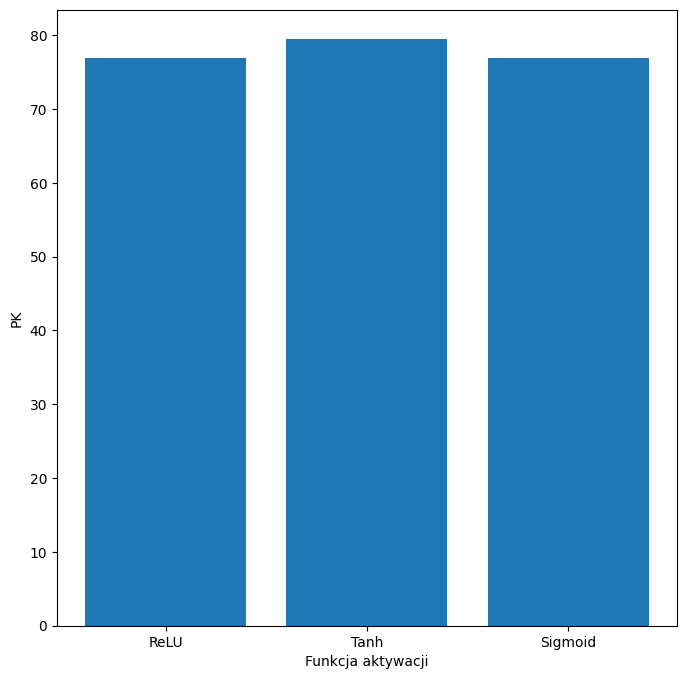
\includegraphics[width=0.8\textwidth, keepaspectratio]{ACTIVATION_1_1.png}
    \caption{Zależność poprawności klasyfikacji od użytej funkcji przejścia}
    \label{fig:activ_1}
\end{figure}

Po zastosowaniu funkcji tangens hiperboliczny jako funkcji aktywacji, sieć osiągnęła najwyższą poprawność klasyfikacji wynoszącą $79.48\%$.
Różnica w wynikach między pozostałymi funkcjami aktywacji nie była jednak znacząca (wyniosła $2.56\%$).
Skrypt został uruchomiony ponownie, używając tych samych parametrów, jednak wynik okazał się inny.

\begin{figure}[H]
    \centering
    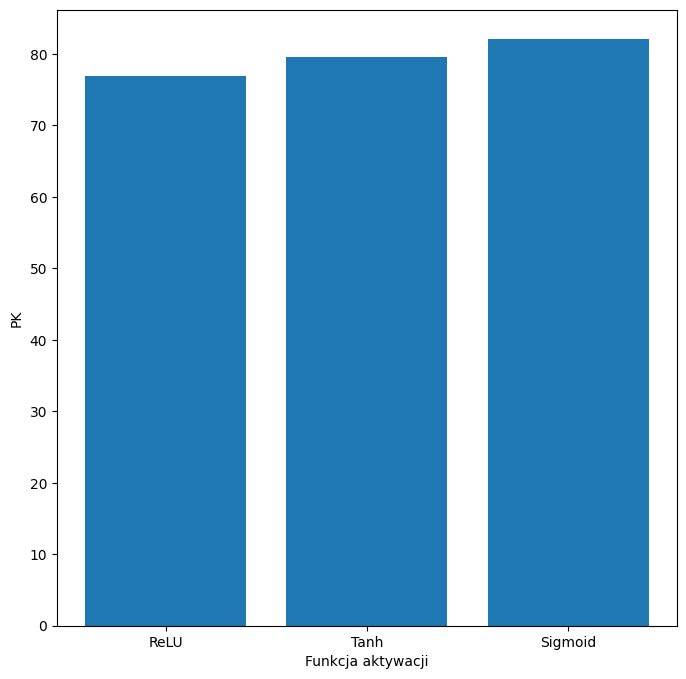
\includegraphics[width=0.8\textwidth, keepaspectratio]{ACTIVATION_1_2.png}
    \caption{Zależność poprawności klasyfikacji od użytej funkcji przejścia}
    \label{fig:activ_2}
\end{figure}

Najwyższą poprawność klasyfikacji osiągnięto przy użyciu funkcji sigmoidalnej, która wynosiła $82\%$.
Tangens hiperboliczny miał poprawność klasyfikacji na poziomie $79.48\%$, natomiast funkcja ReLU osiągnęła wynik $76.92\%$.
Powodem zmiany względem poprzedniego wyniku może być losowy początkowy dobór wag, który ma miejsce podczas inicjalizacji sieci.
To sugeruje, że w tym przypadku funkcja aktywacji nie odgrywa tak istotnej roli.

\newpage
\subsection{Eksperyment 8}
Możliwe, że wynik ulegnie zmianie, gdy zwiększona zostanie liczba warstw i liczba neuronów w sieci.
W ósmym eksperymencie liczba warstw wynosić będzie 5, a liczba neuronów dla każdej warstwy będzie wynosić 100.
Współczynnik uczenia będzie wynosił 0.1, a liczba epok zostanie zwiększona do 1000.

\begin{figure}[H]
    \centering
    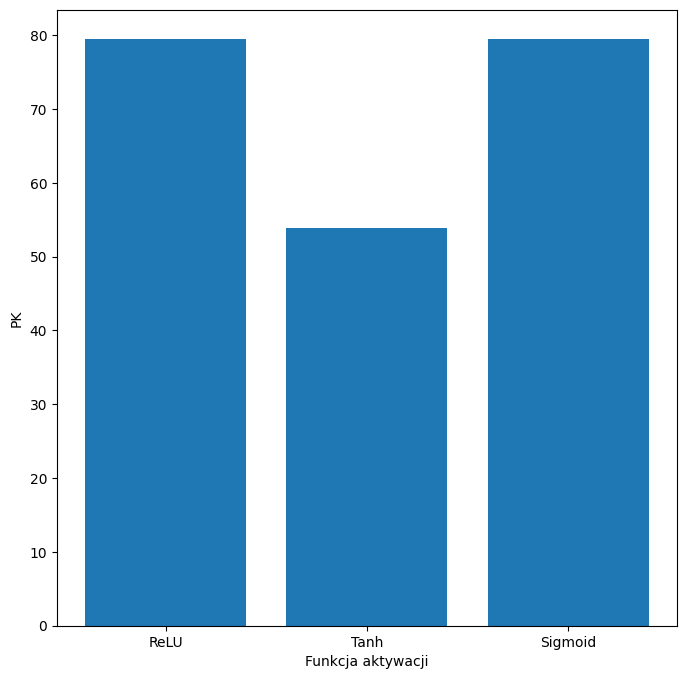
\includegraphics[width=0.8\textwidth, keepaspectratio]{ACTIVATION_2_1.png}
    \caption{Zależność poprawności klasyfikacji od użytej funkcji przejścia}
    \label{fig:activ_2}
\end{figure}

W tym przypadku użyta funkcja aktywacji ma ogromne znaczenie.
Tangens hiperboliczny osiągnął bardzo niski wynik poprawności klasyfikacji na poziomie $53.84\%$.
Natomiast funkcja ReLU oraz sigmoidalna uzyskały identyczny wynik wynoszący $79.48\%$.
Po ponownym uruchomieniu skryptu, tangens hiperboliczny znowu uzyskał najniższą poprawność klasyfikacji.
Wynika z tego, że dla tych parametrów, dla warstw ukrytych najlepiej użyć funkcji ReLU lub funkcji sigmoidalnej.

\newpage
\section{Wnioski}
Na podstawie przeprowadzonych eksperymentów można było dostrzec różne zachowania sieci w zależności od dobranych parametrów.

W eksperymencie pierwszym zaobserwowano, że dla określonych parametrów sieć neuronowa może wykazywać chaotyczne zachowanie.
Jednakże, w porównaniu do pozostałych eksperymentów, w pierwszym eksperymencie osiągnięto najwyższą skuteczność klasyfikacji na poziomie około $94\%$.
Ustawienia można było dobrać również w taki sposób, że rozmiar warstw w sieci nie miał dużego wpływu na poprawność klasyfikacji, która utrzymywała się na podobnym poziomie.
Liczba neuronów w warstwie miała jednak ogromny wpływ jeżeli chodzi o szybkość nauki.
Po zwiększeniu tej liczby w eksperymencie drugim oraz później w trzecim, czas oczekiwania na koniec działania skryptu wzrósł kilkunastokrotnie względem pierwszego.

Dzięki kolejnym eksperymentom można było zauważyć, że zmniejszanie współczynnika uczenia z jednoczesnym zwiększaniem liczby warstw ma tendencję do zmniejszania stabilności sieci.
Można wyciągnąć wniosek, że optymalne wyniki sieć uzyskiwała dla umiarkowanych wartości współczynnika uczenia i liczby warstw.

Następne eksperymenty wykazały, że dla pewnych parametrów, wybór funkcji aktywacji ma istotny wpływ na poprawność klasyfikacji.
Najlepsze wyniki osiągnięto przy użyciu funkcji ReLU lub funkcji sigmoidalnej.
Należy jednak pamiętać, że dla różnych kombinacji liczby warstw i neuronów wyniki mogą być całkowicie inne.

Podsumowując, w większości przypadków rozmiar warstw, współczynnik uczenia, liczba warstw oraz funkcja aktywacji mają wpływ na działanie sieci.
Optymalne wartości tych parametrów będą różnić się w zależności od konkretnego zadania i zbioru danych.
Aby wybrać optymalne wartości wyżej wymienionych parametrów należy przeprowadzić wiele eksperymentów i dokładnie przeanalizować ich wyniki.

\newpage
\section{Dodatki}
\subsection{Pełna część kodu służącego do badania zależności PK od liczby neuronów K1 oraz K2}
\begin{verbatim}
class Model(nn.Module):
    def __init__(self, input_dim, output_dim, K1, K2):
        super(Model, self).__init__()
        self.layer1 = nn.Linear(input_dim, K1)
        self.layer2 = nn.Linear(K1, K2)
        self.layer3 = nn.Linear(K2, output_dim)

    def forward(self, x):
        x = F.relu(self.layer1(x))
        x = F.relu(self.layer2(x))
        x = F.sigmoid(self.layer3(x))
        return x


lr_vec = np.array([1e-1, 1e-2, 1e-3, 1e-4, 1e-5, 1e-6, 1e-7])
K1_vec = np.arange(100, 5000, 100)
K2_vec = K1_vec
PK_2D_K1K2 = np.zeros([len(K1_vec), len(K2_vec)])
max_epoch = 100
PK_2D_K1K2_max = 0
k1_ind_max = 0
k2_ind_max = 0
X_train = Variable(torch.from_numpy(X_train)).float()
y_train = Variable(torch.from_numpy(y_train)).long()
X_test = Variable(torch.from_numpy(X_test)).float()
y_test = Variable(torch.from_numpy(y_test)).long()
for k1_ind in range(len(K1_vec)):
    for k2_ind in range(len(K2_vec)):
        model = Model(X_train.shape[1], int(
            max(y) + 1), K1_vec[k1_ind], K2_vec[k2_ind])
        optimizer = torch.optim.Adam(model.parameters(), lr=lr_vec[1])
        loss_fn = nn.CrossEntropyLoss()

        for epoch in range(max_epoch):
            y_pred = model(X_train)
            loss = loss_fn(y_pred, y_train)

            optimizer.zero_grad()
            loss.backward()
            optimizer.step()

        with torch.no_grad():
            y_pred = model(X_test)
            correct = (torch.argmax(y_pred, dim=1) ==
                       y_test).type(torch.FloatTensor)
            PK = correct.mean().item() * 100
            print("K1 {} | K2 {} | PK {} ".format(
                K1_vec[k1_ind], K2_vec[k2_ind], PK))
            PK_2D_K1K2[k1_ind, k2_ind] = PK

        if PK > PK_2D_K1K2_max:
            PK_2D_K1K2_max = PK
            k1_ind_max = k1_ind
            k2_ind_max = k2_ind

print(K1_vec[k1_ind_max], K2_vec[k2_ind_max], PK_2D_K1K2_max)
fig = plt.figure(figsize=(8, 8))
ax = fig.add_subplot(111, projection="3d")
X, Y = np.meshgrid(K1_vec, K2_vec)
surf = ax.plot_surface(X, Y, PK_2D_K1K2.T, cmap="viridis")
ax.set_xlabel("K1")
ax.set_ylabel("K2")
ax.set_zlabel("PK")
ax.view_init(30, 200)
plt.savefig("Fig.1_PK_K1K2_pytorch_parkinsons.png", bbox_inches="tight")
\end{verbatim}

\newpage
\subsection{Pełna część kodu służącego do badania zależności PK od liczby warstw i współczynniku uczenia}
\begin{verbatim}
class Model(nn.Module):
    def __init__(self, input_dim, output_dim, K):
        super(Model, self).__init__()
        layers = [nn.Linear(input_dim, K[0])]
        for i in range(len(K) - 1):
            layers.append(nn.Linear(K[i], K[i + 1]))
        layers.append(nn.Linear(K[-1], output_dim))
        self.layers = nn.ModuleList(layers)

    def forward(self, x):
        for layer in self.layers[:-1]:
            x = F.relu(layer(x))
        x = F.sigmoid(self.layers[-1](x))
        return x

lr_vec = np.array([1e-1, 1e-2, 1e-3, 1e-4, 1e-5, 1e-6, 1e-7])
K1 = 6
K2 = 4
max_layers = 10
PK_3D_K = np.zeros((len(lr_vec), max_layers))
max_epoch = 100
PK_max = 0
lr_max_ind = 0
layers_for_max_PK = 0

X_train = Variable(torch.from_numpy(X_train)).float()
y_train = Variable(torch.from_numpy(y_train)).long()
X_test = Variable(torch.from_numpy(X_test)).float()
y_test = Variable(torch.from_numpy(y_test)).long()

for lr_ind in range(len(lr_vec)):
    for i in range(3, max_layers + 1):
        layers = []
        for j in range(i):
            if j % 2 == 0:
                layers.append(K1)
            else:
                layers.append(K2)
        model = Model(X_train.shape[1], int(max(y) + 1), layers)
        optimizer = torch.optim.Adam(model.parameters(), lr=lr_vec[lr_ind])
        loss_fn = nn.CrossEntropyLoss()

        for epoch in range(max_epoch):
            y_pred = model(X_train)
            loss = loss_fn(y_pred, y_train)

            optimizer.zero_grad()
            loss.backward()
            optimizer.step()

        with torch.no_grad():
            y_pred = model(X_test)
            correct = (torch.argmax(y_pred, dim=1) == y_test).type(torch.FloatTensor)
            PK = correct.mean().item() * 100
            print(
                "LR {} | K1 {} | K2 {} | PK {} | layers {} | layers_count {} ".format(
                    lr_vec[lr_ind], K1, K2, PK, layers, len(layers)
                )
            )
            PK_3D_K[lr_ind, i - 3] = PK

        if PK > PK_max:
            PK_max = PK
            lr_max_ind = lr_ind
            layers_for_max_PK = len(layers)

print(
    "Max PK: {} for LR: {} | K1: {} | K2: {} | layers_count {} ".format(
        PK_max, lr_vec[lr_max_ind], K1, K2, layers_for_max_PK
    )
)

PK_3D_K = PK_3D_K[:, : max_layers - 2]
fig = plt.figure(figsize=(8, 8))
ax = fig.add_subplot(111, projection="3d")
Y, X = np.meshgrid(np.log10(lr_vec), np.array([range(3, max_layers + 1)]))
ax.plot_surface(X, Y, PK_3D_K.T, cmap="viridis")
ax.set_xlabel("Liczba warstw")
ax.set_ylabel("Współczynnik uczenia (10^x)")
ax.set_zlabel("PK")
plt.savefig("Fig.1_PK_layers_lr_pytorch_parkinsons.png", bbox_inches="tight")
plt.show()

\end{verbatim}
\newpage
\subsection{Pełna część kodu służącego do badania zależności PK od użytej funkcji aktywacji}
\begin{verbatim}
class Model(nn.Module):
    def __init__(self, input_dim, output_dim, K, activation):
        super(Model, self).__init__()
        layers = [nn.Linear(input_dim, K[0])]
        for i in range(len(K) - 1):
            layers.append(nn.Linear(K[i], K[i+1]))
        layers.append(nn.Linear(K[-1], output_dim))
        self.layers = nn.ModuleList(layers)
        self.activation = activation

    def forward(self, x):
        for layer in self.layers[:-1]:
            x = self.activation(layer(x))
        x = F.softmax(self.layers[-1](x), dim=1)
        return x

activations = [F.relu, F.tanh, F.sigmoid]
PK_activations = []
layers = 5
max_epoch = 1000
K = [100, 100, 100, 100, 100]
X_train = Variable(torch.from_numpy(X_train)).float()
y_train = Variable(torch.from_numpy(y_train)).long()
X_test = Variable(torch.from_numpy(X_test)).float()
y_test = Variable(torch.from_numpy(y_test)).long()
lr_vec = np.array([1e-1, 1e-2, 1e-3, 1e-4, 1e-5, 1e-6, 1e-7])
for activation in activations:
    model = Model(X_train.shape[1], int(max(y) + 1), K, activation)
    optimizer = torch.optim.Adam(model.parameters(), lr=lr_vec[0])
    loss_fn = nn.CrossEntropyLoss()

    for epoch in range(max_epoch):
        y_pred = model(X_train)
        loss = loss_fn(y_pred, y_train)

        optimizer.zero_grad()
        loss.backward()
        optimizer.step()

    with torch.no_grad():
        y_pred = model(X_test)
        correct = (torch.argmax(y_pred, dim=1) == y_test).type(torch.FloatTensor)
        PK = correct.mean().item() * 100
        PK_activations.append(PK)
        print("PK {} FUNCTION {}".format(PK, activation))

fig = plt.figure(figsize=(8, 8))
ax = fig.add_subplot()
ax.bar(['ReLU', 'Tanh', 'Sigmoid'], PK_activations)
ax.set_xlabel('Funkcja aktywacji')
ax.set_ylabel('PK')
plt.savefig("Fig.2_PK_activations_pytorch_parkinsons.png", bbox_inches="tight")
plt.show()
\end{verbatim}

\newpage
\begin{thebibliography}{9}
    \bibitem{Nielsen}
    Michael Nielsen,
    \emph{Neural Networks and Deep Learning}.
    Determination Press,
    2015.
    \bibitem{TadeusiewiczSzaleniec}
    Ryszard Tadeusiewicz, Maciej Szaleniec,
    \emph{Leksykon sieci neuronowych}.
    Wrocław,
    2015.
    \bibitem{zajdel}
    Zajdel R.,
    \emph{Ćwiczenie 4 Model Neuronu},
    Rzeszów,
    KIiA, PRz.
    \bibitem{gora}
    Paweł Gora,
    \href{https://www.deltami.edu.pl/temat/informatyka/sztuczna_inteligencja/2017/12/28/Glebokie_uczenie_maszyn/}{\emph{Głębokie uczenie maszyn}},
    [dostęp: 17.05.2023].
    \bibitem{zajdel}
    Zajdel R.,
    \emph{Procedura przygotowania danych dla sieci neuronowych na potrzeby projektu z modułu sztuczna inteligencja - Listing1},
    Rzeszów,
    KIiA, PRz.
    \bibitem{zajdel}
    Zajdel R.,
    \emph{Procedura przygotowania danych dla sieci neuronowych na potrzeby projektu z modułu sztuczna inteligencja - Listing2},
    Rzeszów,
    KIiA, PRz.
\end{thebibliography}
\end{document}